\renewcommand{\EntradaBibtex}{2025_FlipAnim_Euresti_Junior}

% Metadata
%\title[FlipAnim Mobile]{Adaptación Móvil de FlipAnim en Jetpack Compose}
%\subtitle{Desarrollo de Aplicaciones Móviles -- Unidad 2}
%\author[C. Euresti, D. Ramírez, J. Vázquez, D. Zapata]{%
%  César Euresti \and Diego Ramírez Ibarra \\
%  Junior Arturo Vázquez Leonel* \and Diego Eduardo Zapata Aguilar*
%}

% -----------------------------------------------------------------------------
% SLIDE 2: Introducción y Justificación
% -----------------------------------------------------------------------------
\begin{frame}{\citetitle{\EntradaBibtex}$^*$ (1)}
%\begin{block}{Introducción y Justificación}

  \begin{columns}[T]
    \begin{column}{0.48\textwidth}
      \begin{block}{El Problema}
        \begin{itemize}
          \item \textbf{FlipAnim Web} permite crear animaciones 2D \emph{frame-by-frame} con una interfaz minimalista.
          \item La versión web resulta \textbf{limitada en dispositivos móviles} (latencia táctil, falta de persistencia local y restricciones en la exportación).
        \end{itemize}
      \end{block}
      
      %\begin{block}{Objetivo Principal}
      %  Desarrollar una \textbf{aplicación nativa Android} que replique el flujo ágil de FlipAnim optimizado para pantallas táctiles y lápiz óptico.
      %\end{block}
    \end{column}

    \begin{column}{0.48\textwidth}
      \begin{block}{Objetivo Principal}
            Desarrollar una \textbf{aplicación nativa Android} que replique el flujo ágil de FlipAnim optimizado para pantallas táctiles y lápiz óptico.
      \end{block}
    \end{column}
  \end{columns}
%\end{block}
\footfullcite*{\EntradaBibtex}
\end{frame}

% -----------------------------------------------------------------------------
% SLIDE 3: Arquitectura y Contribuciones Técnicas
% -----------------------------------------------------------------------------
%\begin{frame}{2. Arquitectura y Modelo de Datos}
\begin{frame}{\citetitle{\EntradaBibtex} (2)}
  \begin{columns}[T]
    \begin{column}{0.5\textwidth}
      \begin{block}{Estructura Jerárquica del Estado}
        \begin{itemize}
          \item \textbf{Project:} Contenedor global (lista de fotogramas, paleta cromática, ID activo).
          \item \textbf{Frame:} Duración (ms), capas y pila de deshacer/rehacer (\texttt{UndoStack}).
          \item \textbf{Layer:} Visibilidad, orden y jerarquía de dibujables.
          \item \textbf{Drawable (Interfaz Sellada):}
            \begin{itemize}
              \item \texttt{Stroke}: Trazos libres vectoriales.
              \item \texttt{FillPath}: Rellenos de región.
              \item \texttt{Primitive}: Figuras geométricas.
            \end{itemize}
        \end{itemize}
      \end{block}
    \end{column}

    \begin{column}{0.46\textwidth}
      \begin{block}{Contribuciones Técnicas Clave}
        \begin{enumerate}
          \item \textbf{Persistencia y Serialización:} Modelo completo convertible a formato JSON (\texttt{ProjectJson}).
          \item \textbf{Primitivas Estilo Paint:} Formas geométricas parametrizables con controles de trazo y relleno.
          \item \textbf{Exportación Multimedia:} Motor fuera de pantalla renderizado con \texttt{MediaCodec} (H.264/MP4) y \texttt{GifEncoder}.
        \end{enumerate}
      \end{block}
    \end{column}
  \end{columns}
\end{frame}

% -----------------------------------------------------------------------------
% SLIDE 4: Funcionalidades del Motor de Animación
% -----------------------------------------------------------------------------
\begin{frame}{\citetitle{\EntradaBibtex} (3)}
  \begin{columns}[T]
    \begin{column}{0.48\textwidth}
      \begin{block}{Piel de Cebolla (Onion Skinning)}
        \begin{itemize}
          \item Módulo \texttt{OnionSkinOverlay} para ver fotogramas adyacentes.
          \item Renderizado semitransparente con \texttt{ColorFilter.tint}.
          \item Permite mantener la continuidad cinemática entre pose y pose.
        \end{itemize}
      \end{block}

      \begin{block}{Sistema de Reproducción}
        \begin{itemize}
          \item Controlado mediante \texttt{LaunchedEffect} y corrutinas.
          \item Actualización del índice según la duración especificada de cada frame.
          \item Manejo automático de pausas y ciclos de vida del ciclo Android.
        \end{itemize}
      \end{block}
    \end{column}

    \begin{column}{0.48\textwidth}
      \begin{block}{Optimización del Renderizado}
        \begin{itemize}
          \item Coordenadas lógicas fijas ($1024 \times 768$) independientes de la resolución del dispositivo.
          \item Captura de gestos táctiles mediante \texttt{pointerInput} y \texttt{awaitEachGesture}.
          \item Reutilización de objetos \texttt{Path} mediante \texttt{remember} y \texttt{reset()} para evitar sobrecarga del \emph{Garbage Collector}.
        \end{itemize}
      \end{block}
    \end{column}
  \end{columns}
\end{frame}

% -----------------------------------------------------------------------------
% SLIDE 5: Resultados y Conclusión
% -----------------------------------------------------------------------------
\begin{frame}{\citetitle{\EntradaBibtex} (4)}
  \begin{columns}[T]
    \begin{column}{0.52\textwidth}
      \begin{block}{Resultados de la Interfaz}
        \begin{itemize}
          \item \textbf{Lienzo Central:} Área de trabajo maximizada con controles periféricos limpios.
          \item \textbf{Herramientas Inmediatas:} Selección cromática desplegable, ajuste continuo de grosor del pincel y figuras predefinidas.
          \item \textbf{Modo Pantalla Completa:} Maximiza la superficie de dibujo eliminando distracciones.
          \item \textbf{Panel de Exportación:} Configuración de velocidad de fotogramas (FPS) y resolución en MP4/JSON.
        \end{itemize}
      \end{block}
    \end{column}

    \begin{column}{0.44\textwidth}
      \begin{block}{Conclusión}
        Se logró exitosamente una \textbf{adaptación fiel y de alto rendimiento} de FlipAnim para Android, trasladando la experiencia creativa a un entorno táctil gracias a la potencia de \textbf{Jetpack Compose}.
      \end{block}
    \end{column}
  \end{columns}
\end{frame}

\begin{frame}{\citetitle{\EntradaBibtex} (5)}
\begin{block}{Implementación} 
\begin{columns}
\column{.5\linewidth}
\begin{center}
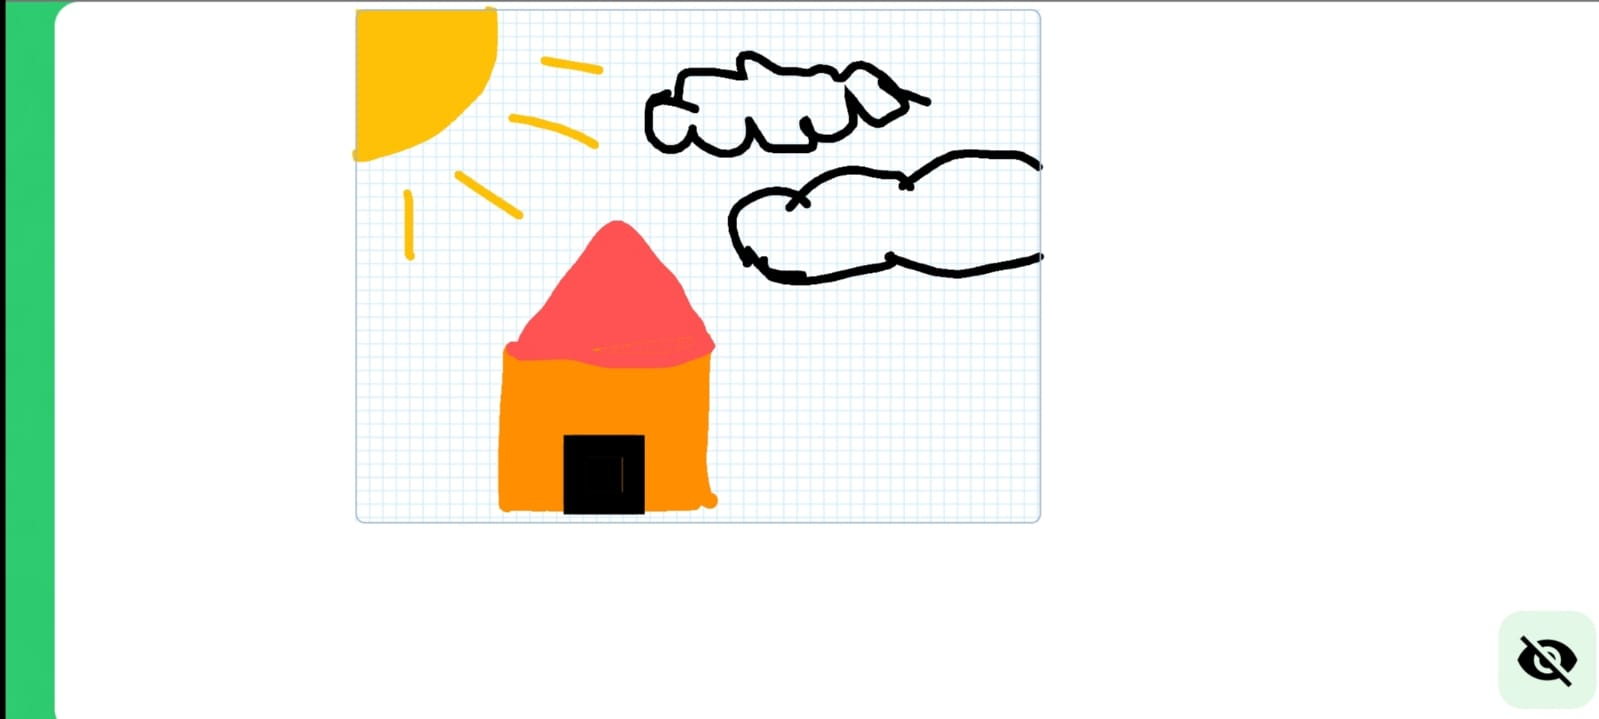
\includegraphics[width=.95\linewidth]{2025_FlipAnim/figs/full_screen_view.jpeg}
\end{center}
\column{.5\linewidth}
\begin{center}
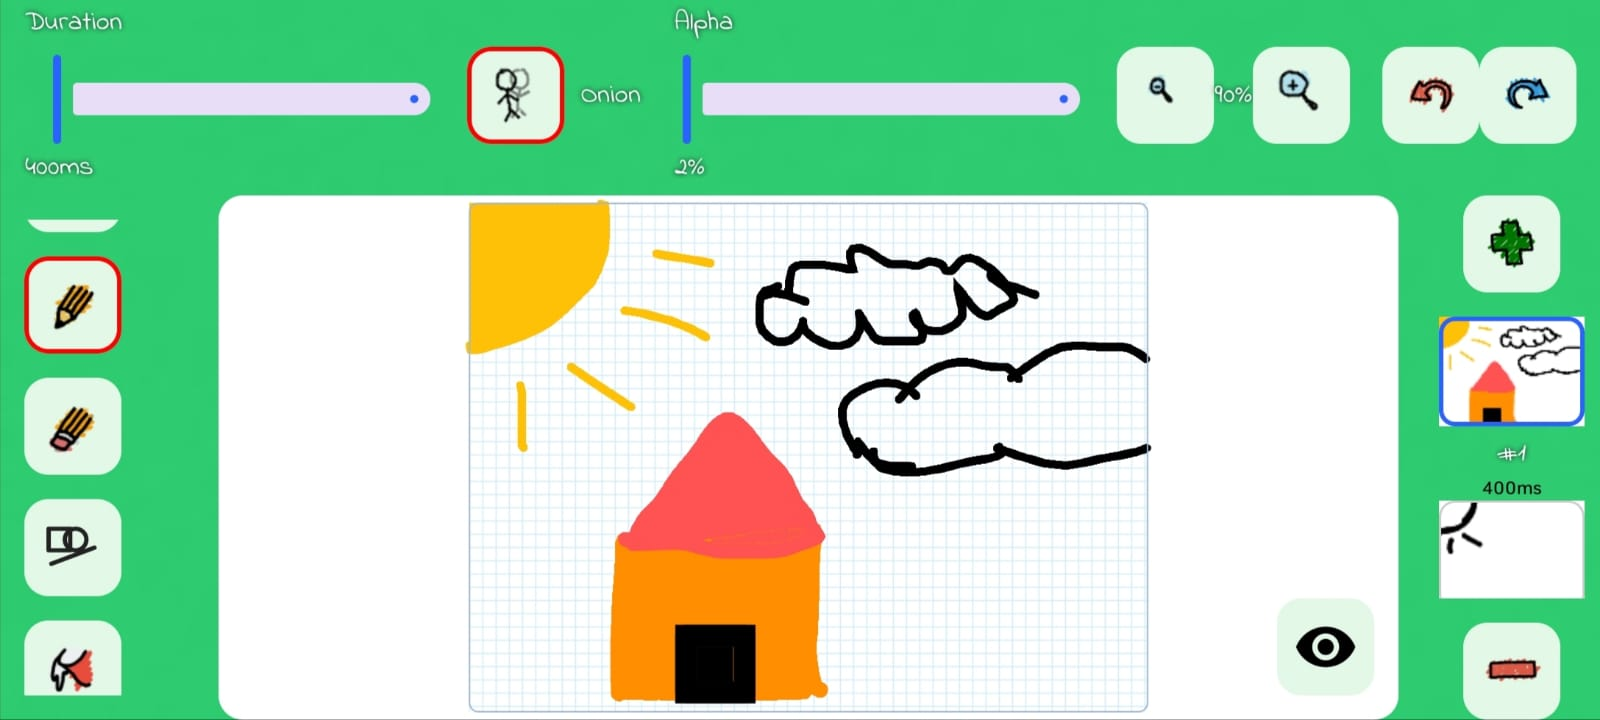
\includegraphics[width=.95\linewidth]{2025_FlipAnim/figs/general_interface.jpeg}
\end{center}
\end{columns}

\end{block} 

\end{frame}


\begin{frame}{\citetitle{\EntradaBibtex} (6)}
\begin{block}{Implementación} 
\begin{columns}
\column{.5\linewidth}
\begin{center}
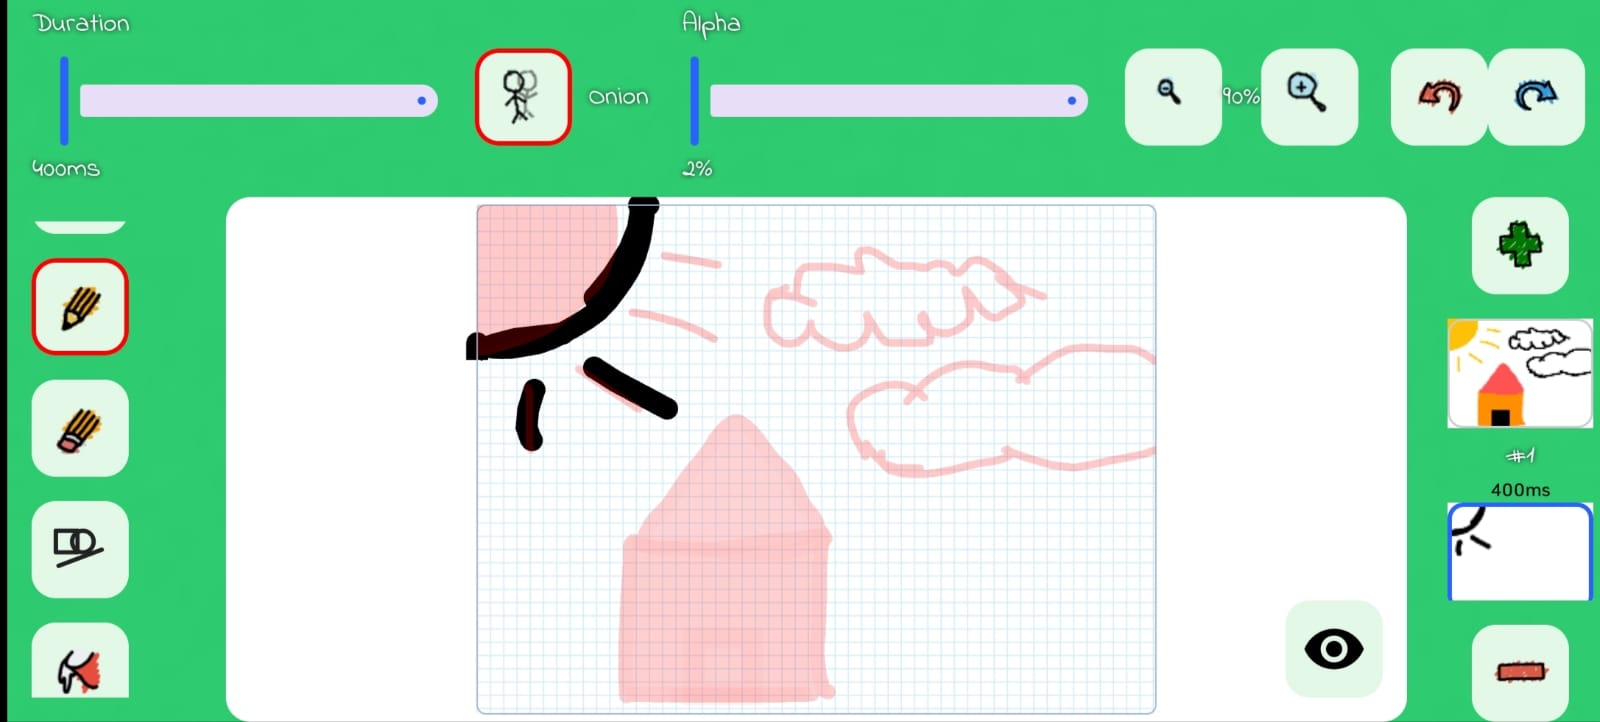
\includegraphics[width=.95\linewidth]{2025_FlipAnim/figs/onion_skin.jpeg}
\end{center}
\column{.5\linewidth}
\begin{center}
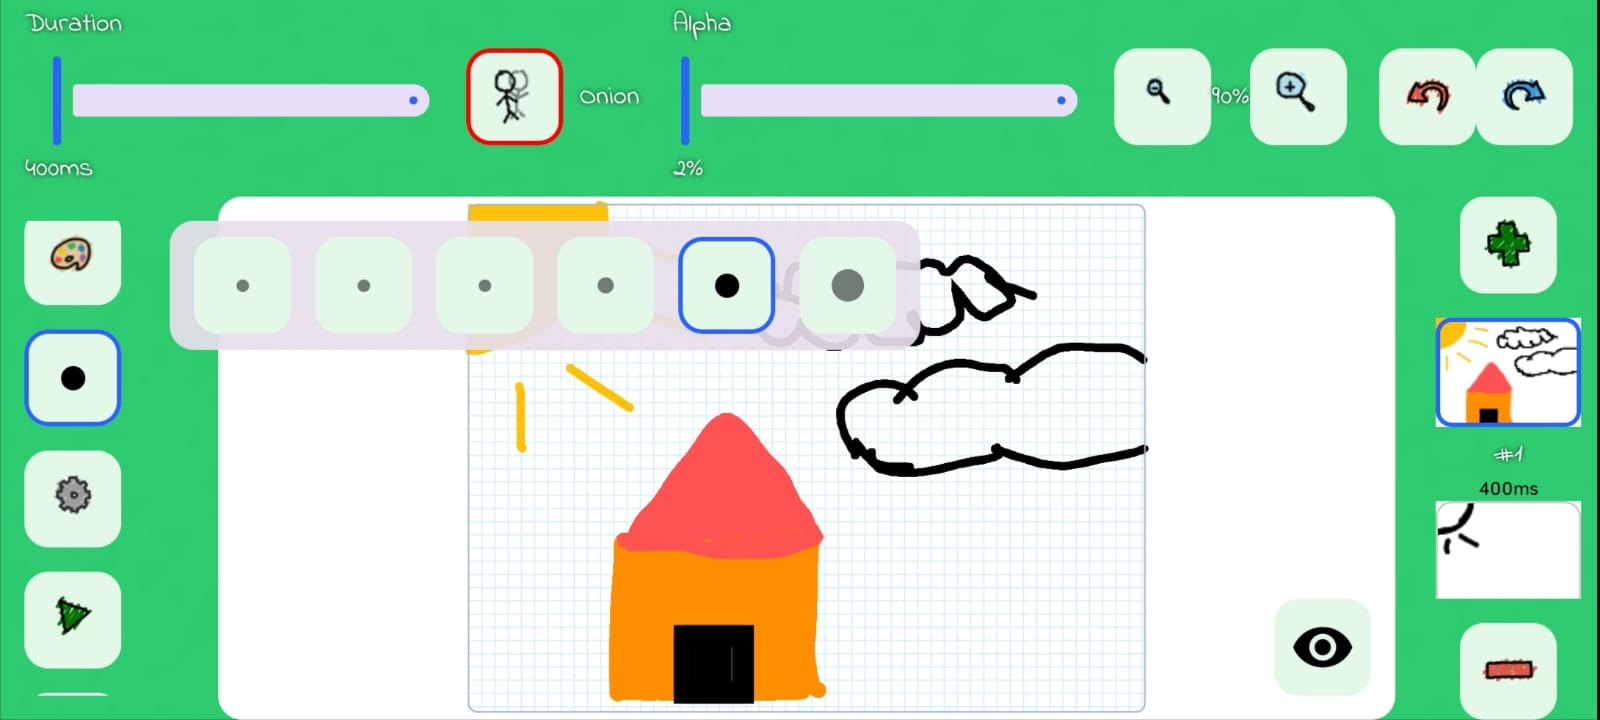
\includegraphics[width=.95\linewidth]{2025_FlipAnim/figs/show_options_pencil_stroke.jpeg}
\end{center}
\end{columns}

\end{block} 

\end{frame}



%
%2025_FlipAnim/figs/show_options_colors.jpeg
%

